\documentclass{IOS-Book-Article}
\usepackage{mathptmx}
\usepackage{hyperref,url}
\usepackage{graphicx}
\usepackage{float}
\def\Eo{\mbox{\sc Ezo}}
\def\Ec{\mbox{\sc Ezo-CNN}}
\def\Mx{\mbox{\sc MoHex}}
\def\Mc{\mbox{\sc MoHex-CNN}}
\def\Mt{\mbox{\sc MoHex-3HNN}}
\def\Sol{\mbox{\sc Solver}}
\def\Fuego{\mbox{\sc Fuego}}

\def\hb{\hbox to 10.7 cm{}}

\begin{document}
\pagestyle{headings}
\def\thepage{}
\begin{frontmatter}              % The preamble begins here.
%\pretitle{Pretitle}
\title{MoHex3HNN defeats EzoCNN in Hex}
\markboth{}{2018 New Taipei City Computer Olympiad Report: to appear in ICGA Journal}
\author{\fnms{Chao} \snm{Gao}} and
\author{\fnms{Kei} \snm{Takada}} and
\author{\fnms{Ryan} \snm{Hayward}\thanks{Corresponding 
  author: hayward@ualberta.ca.}}

\runningauthor{AuthorA et al.}
\address{Department of Computing Science, University of Alberta, Canada}
\end{frontmatter}
\markboth{Gao, Takada, Hayward}{\Mt\ defeats \Ec\ in Hex 2018}

\begin{figure}[hbt]
\includegraphics[width=\columnwidth]{photos/awards.eps}\
\caption{From left, Kei Takada, Chao Gao, Ryan Hayward}
\end{figure}
%convert hex-medallists.jpg -gravity Center -crop 95x66%+0+0 -compress lzw eps2:a.eps

\section{The Tournaments}
There were two Hex tournaments at the 2018 Computer Olympiad in New Taipei City:
board-size 11$\times$11 and 
board-size 13$\times$13.\footnote{\cite{H17olyrptsource} has .sgf 
  game records and source files for this report.
  \cite{Hexgui} has an SGF (Smart Game Format) viewer.
  SGF was developed by \cite{SGF}.}
11$\times$11 Hex is the original game introduced by Piet Hein in 1942. 
All one-move openings on all $n$$\times$$n$ Hex boards up to 9$\times$9
have been solved by computers, as have two 10$\times$10 openings 
\cite{PawlH13}.
11$\times$11 games are typically computer-solved after 25 moves,
so in recent years a 13$\times$13 tournament has been added.

%13 J b2 a3 c12 (b11 a2 c2)
%11 J j2 b4(?) (c2 c10)

The two tournaments had the same two contestants:
\Ec{} from Japan, 
by Kei Takada, supervised by Masahito Yamamoto;
and \Mt{} from Canada,
by Chao Gao, supervised by Ryan Hayward and Martin M\"{u}ller and
assisted by 
Jakub Pawlewicz,
Ashley Herman,
Joseph Meleshko,
Jiahao Li,
Paul Banse,
Siqi Yan,
Wai Yi Low
and
Xutong Zhao.
Gao and Pawlewicz developed a self-play game procedure,
and game statistics were then used to select opening moves.

\Mt\ is an AlphaGo-style neural net program that shares
much code from the earlier MoHex 2.0 by 
Broderick Arneson, Philip Henderson, Aja Huang, 
Jakub Pawlewicz, Noah Weninger, Kenny Young and Ryan Hayward.
MoHex versions
won the previous
eight Olympiad Hex competitions \cite{HAHP13},
TODO REF 2017
is an MCTS program that uses the Benzene Hex framework
built on the code base of \Fuego\ \cite{fuego}.
%the Go program developed by Martin M\"{u}ller, Markus Enzenberger
%and others at the University of Alberta.
%Benzene allows virtual connection and
%inferior cell computations.
\Mx{} performs knowledge computation 
in UCT tree nodes visited at least 256 times.
\Mx{} ran on Firecreek, a 24 core shared-memory machine, 
with four cores reserved for the 
DFPNS solver \cite{PawlH13}, which
produces perfect play if it solves the
position within the time allotted.
\Mx{} uses a book built by Broderick Arneson with Thomas Lincke's method 
\cite{DBLP:conf/cg/Lincke00}. 
Noah Weninger expanded the book and added a feature
allowing the use of rotational symmetry for openings
whose rotation is in the book.
For each board size, the book covers at least eight openings.

\Mt{}, the successor of \Mc,
uses a three-head convolutional neural net (CNN)
with 128 filters per layer \cite{ijcai}
and was trained on 400 000 self-play games.
At each new node of the Monte Carlo search tree, 
the three-headed neural net is called
and returns policy, state, and action values.
\Mt{} ran remotely on a machine with four CPU cores and one GPU.

\Eo{}, based on the Benzene framework, 
uses iterative deepening alpha-beta search 
with policy and value functions
learned from 10 000 000 self-play games
generated by minimax search.
\Ec{} ran remotely on a machine
with two CPUs and one GPU.
In some games the internet connection was dropped
and computation restarted on a  laptop.
with one CPU-thread for search and one CPU-thread for
Benzene's Depth-First Proof Number Search endgame solver.

Each tournament was scheduled for 8 games between
each two of the three competitors, with 30'/game per player.
The 13$\times$13 and 11$\times$11 tournaments were played
on July 8 and 9 respectively.
Each game ended by resignation as soon as an opponent win was detected.

{\bf Tournament results.}
\Mc\ won both best-of-eight competitions by the same score, 5-0.

\section{13$\times$13 Tournament}
In a game, if the second move is `swap', then players
exchange colors and the first player plays the next move:
in the corresponding diagram, black `S' marks the first two moves
and white `3' the next move.
In the figures, `X-Y 1-0' indicates that X plays first, starting as black, 
and X wins (as white if B swapped, as black if not).

\begin{figure}
\noindent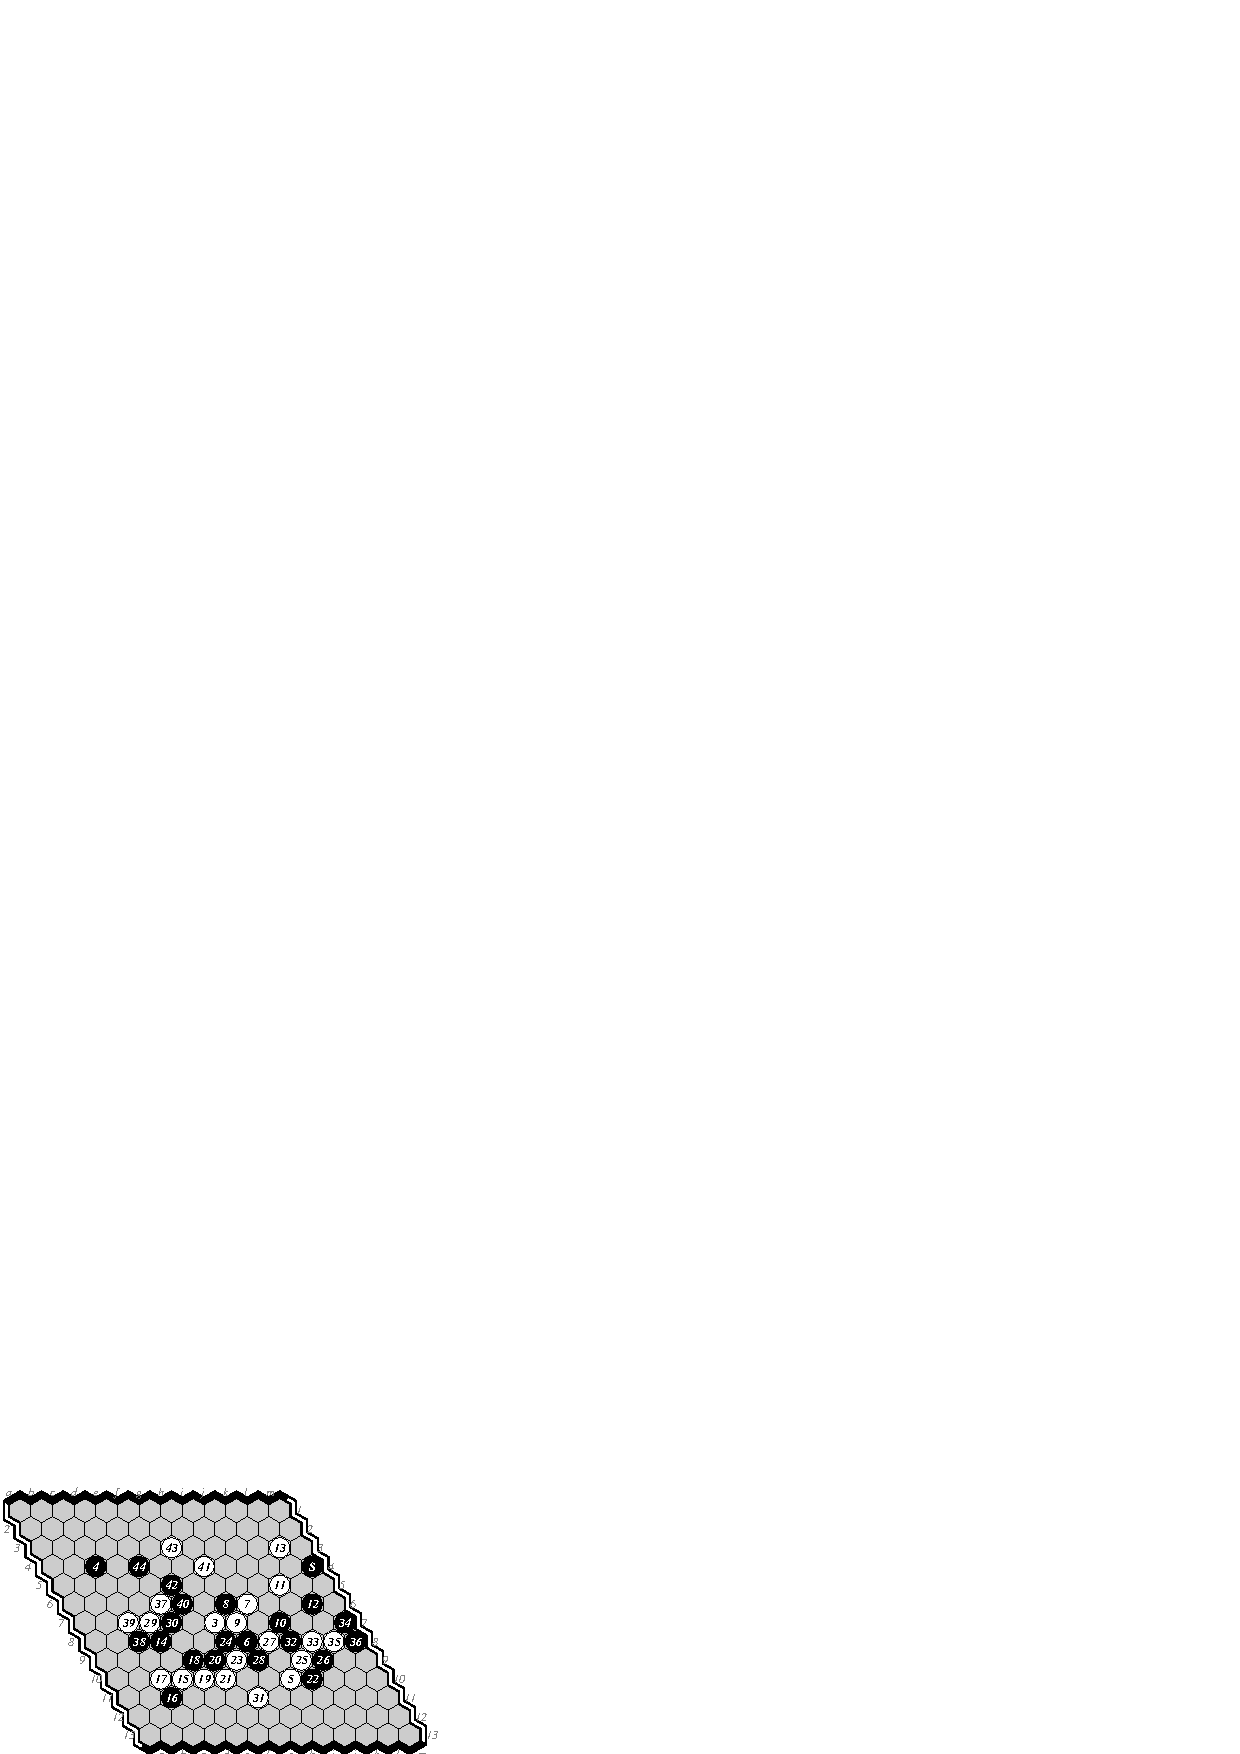
\includegraphics[width=.58\columnwidth]{pix/01-e-m}\hspace*{-.14\columnwidth}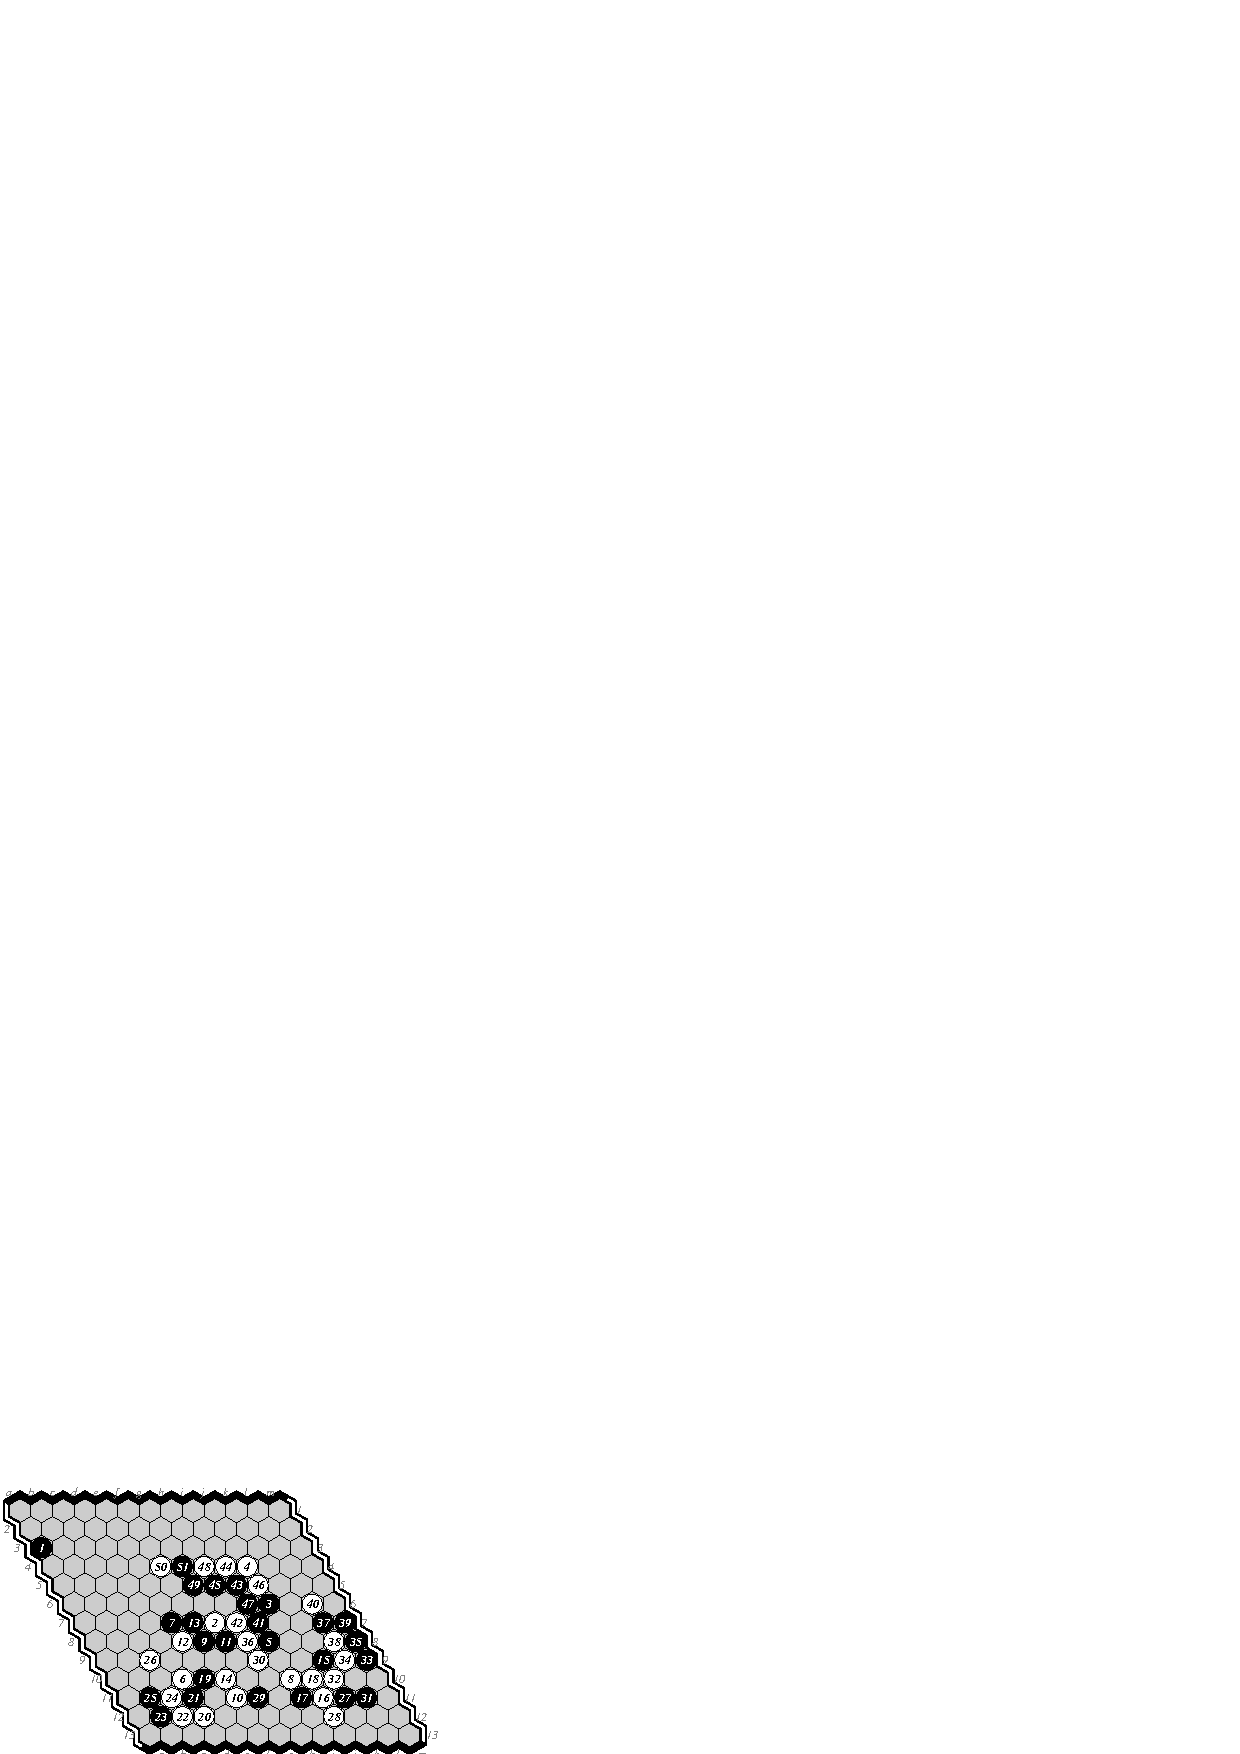
\includegraphics[width=.58\columnwidth]{pix/02-m-e}
\vspace*{.2cm}

\noindent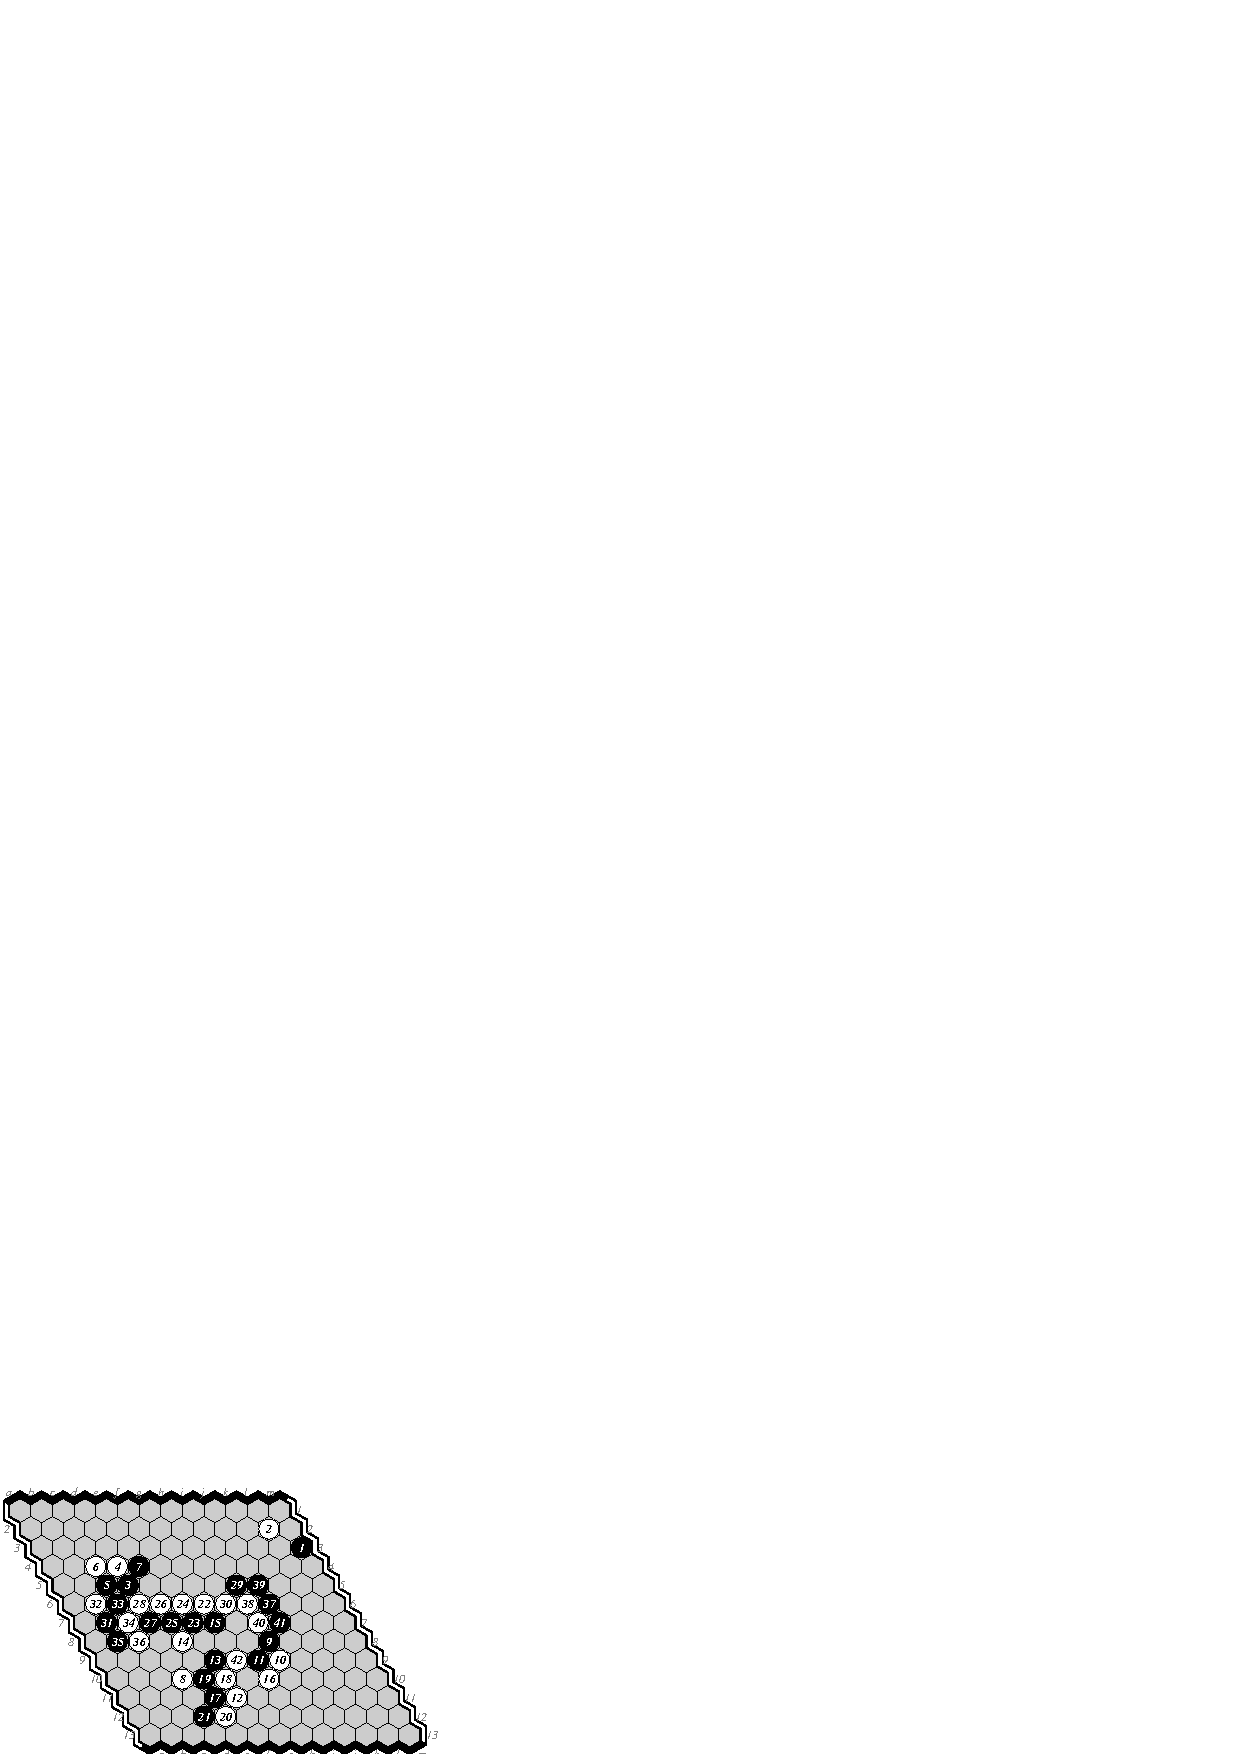
\includegraphics[width=.58\columnwidth]{pix/03-e-m}\hspace*{-.14\columnwidth}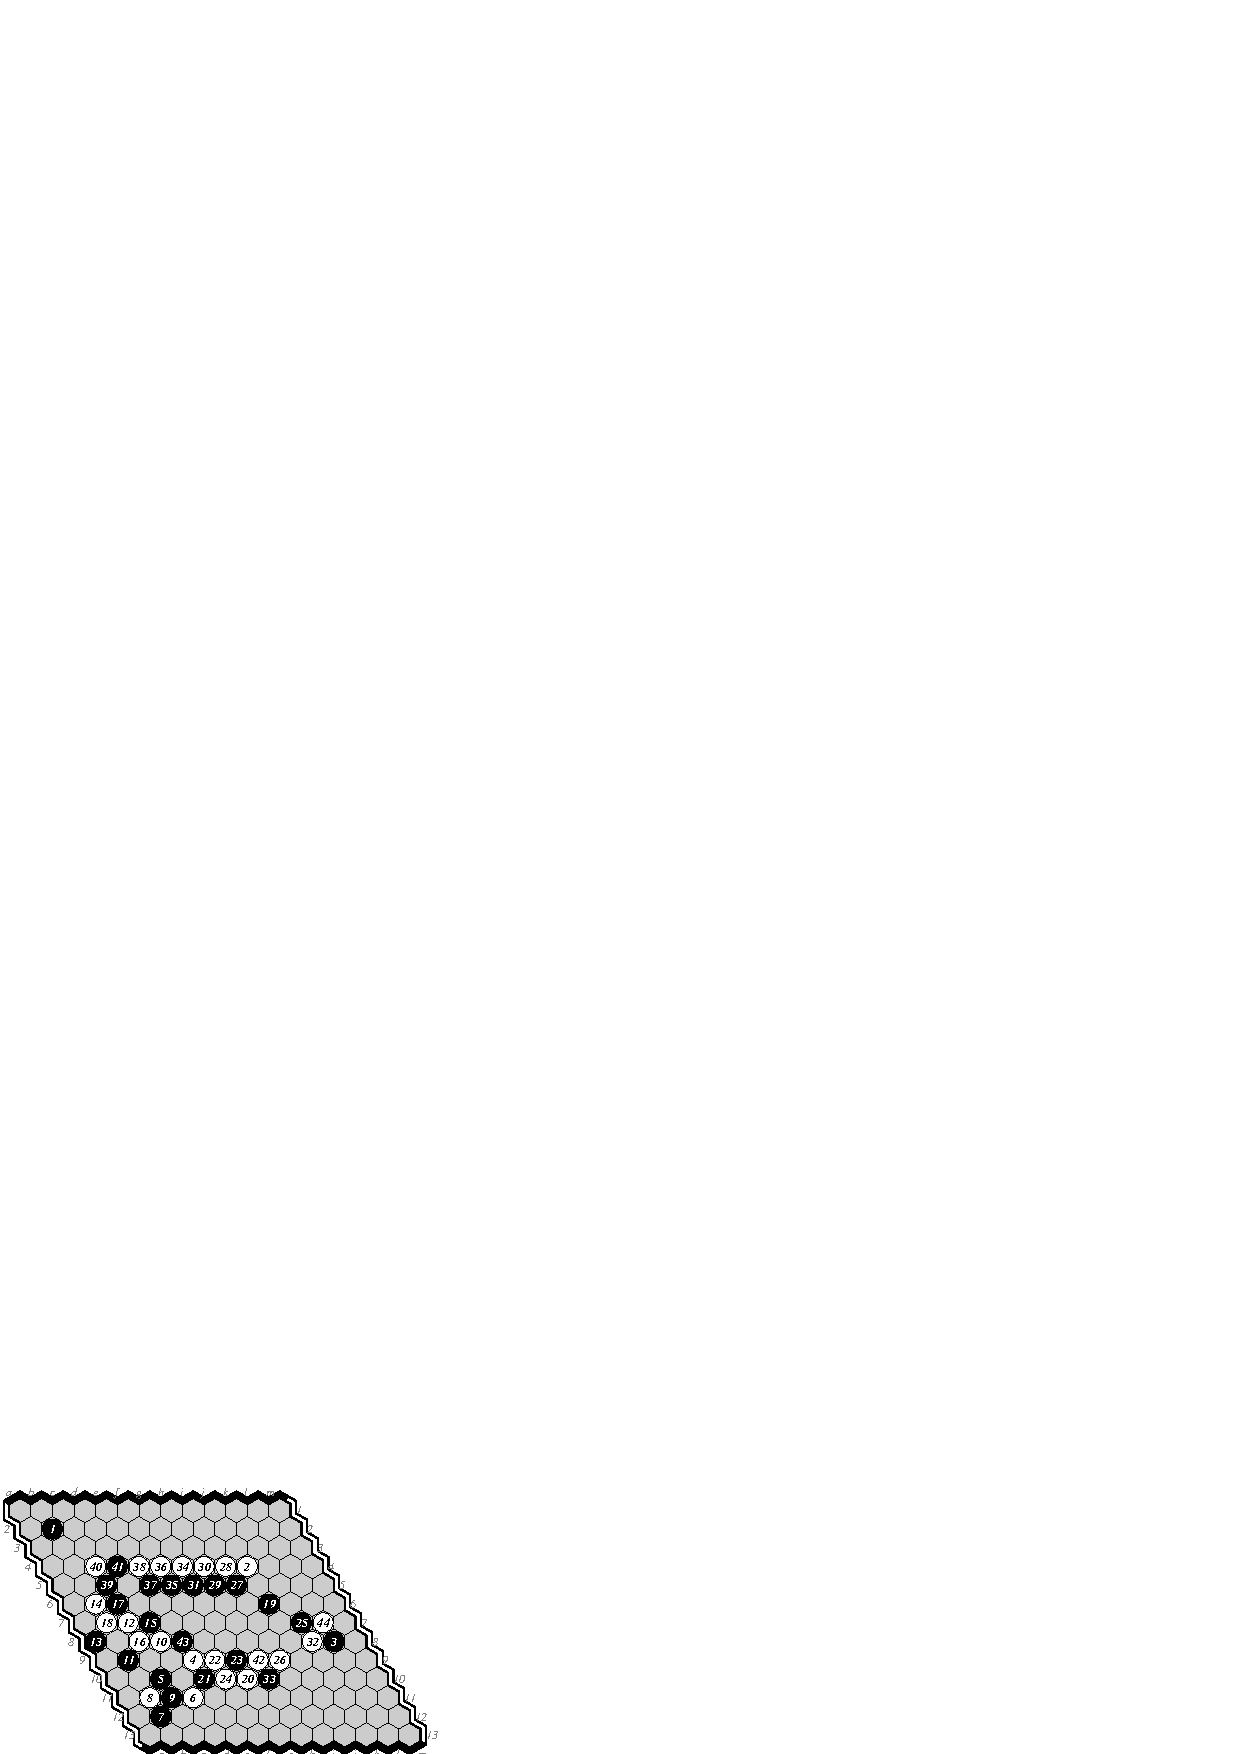
\includegraphics[width=.58\columnwidth]{pix/04-m-e}
\vspace*{.2cm}

\noindent\hfill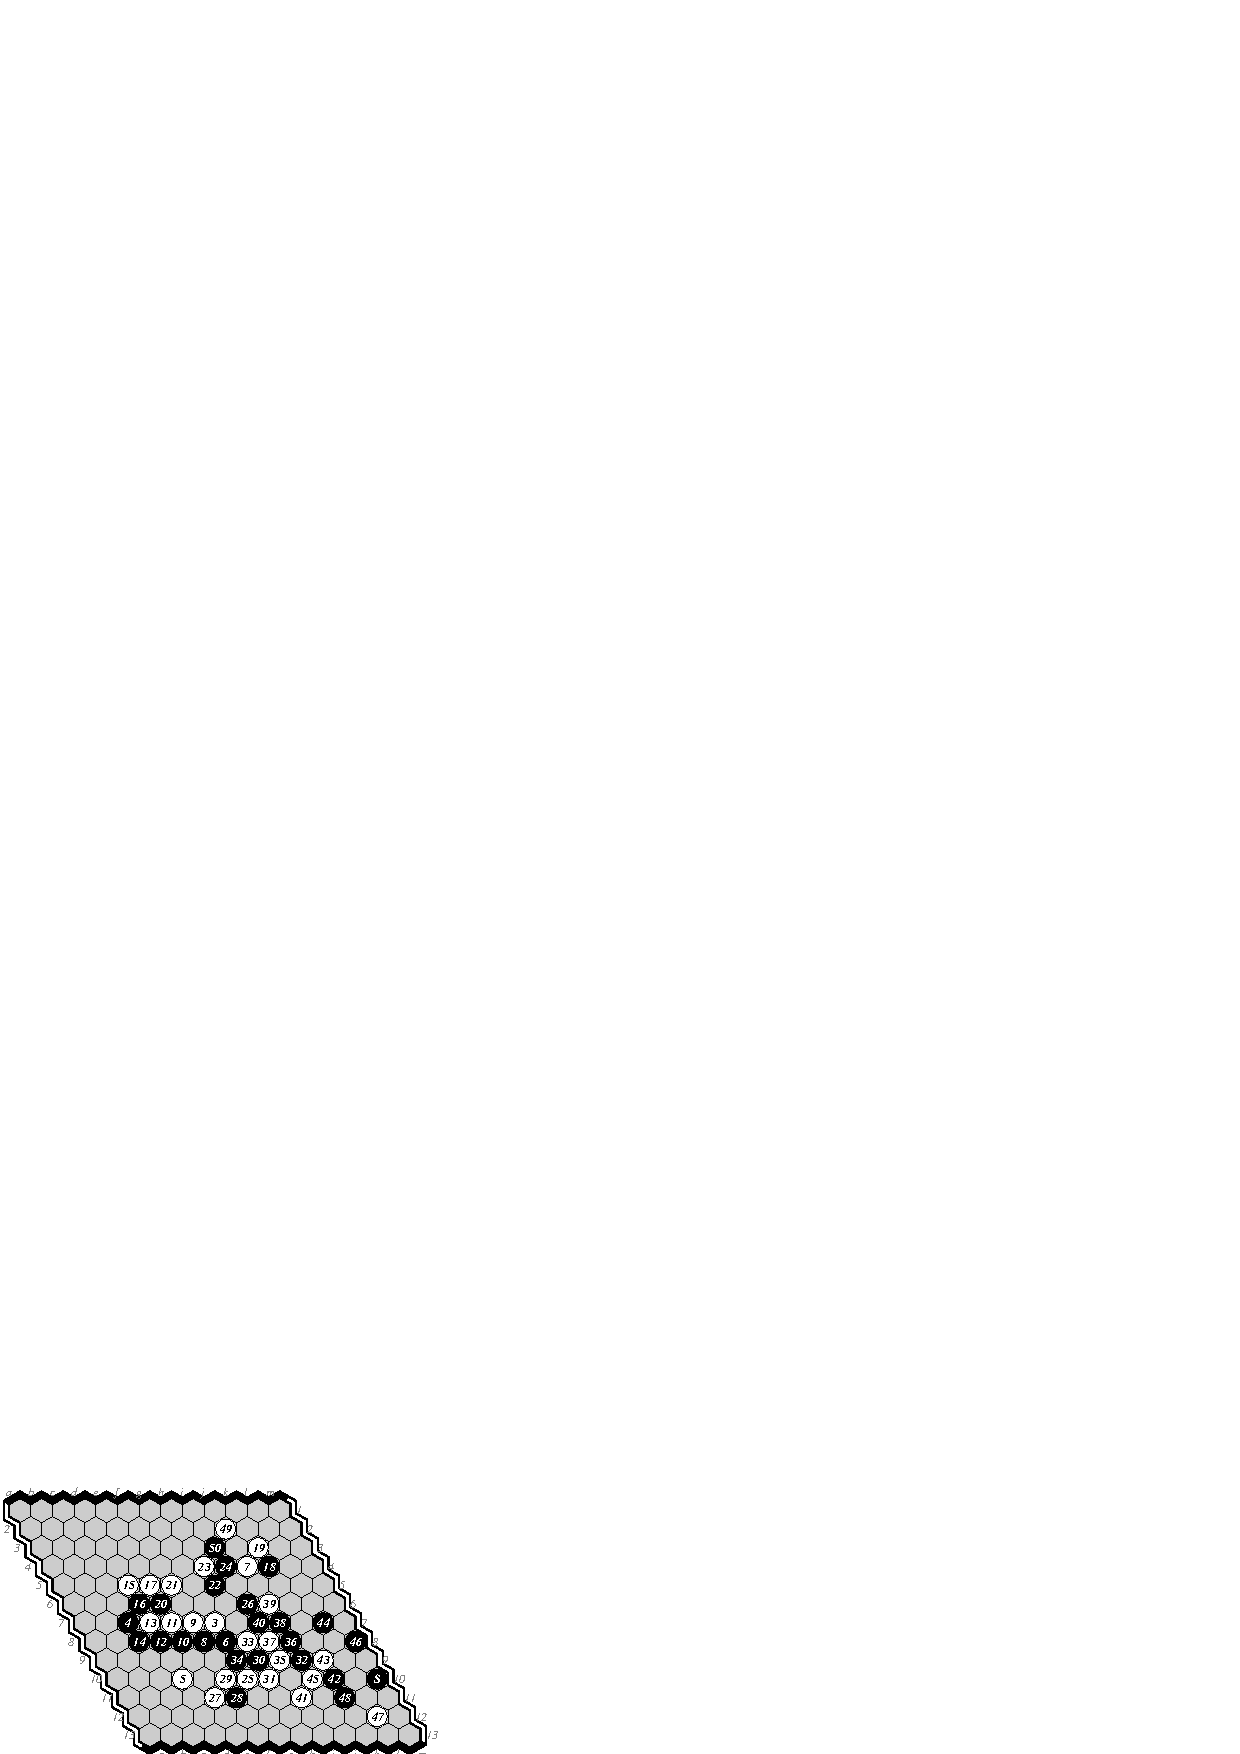
\includegraphics[width=.58\columnwidth]{pix/05-e-m}\hfill\ 
\caption{13$\times$13 Games 1-5. E-M 0-1, M-E 1-0, E-M 0-1, M-E 1-0, E-M 0-1.}
\end{figure}

\section{11$\times$11 Tournament.}
\begin{figure}
\noindent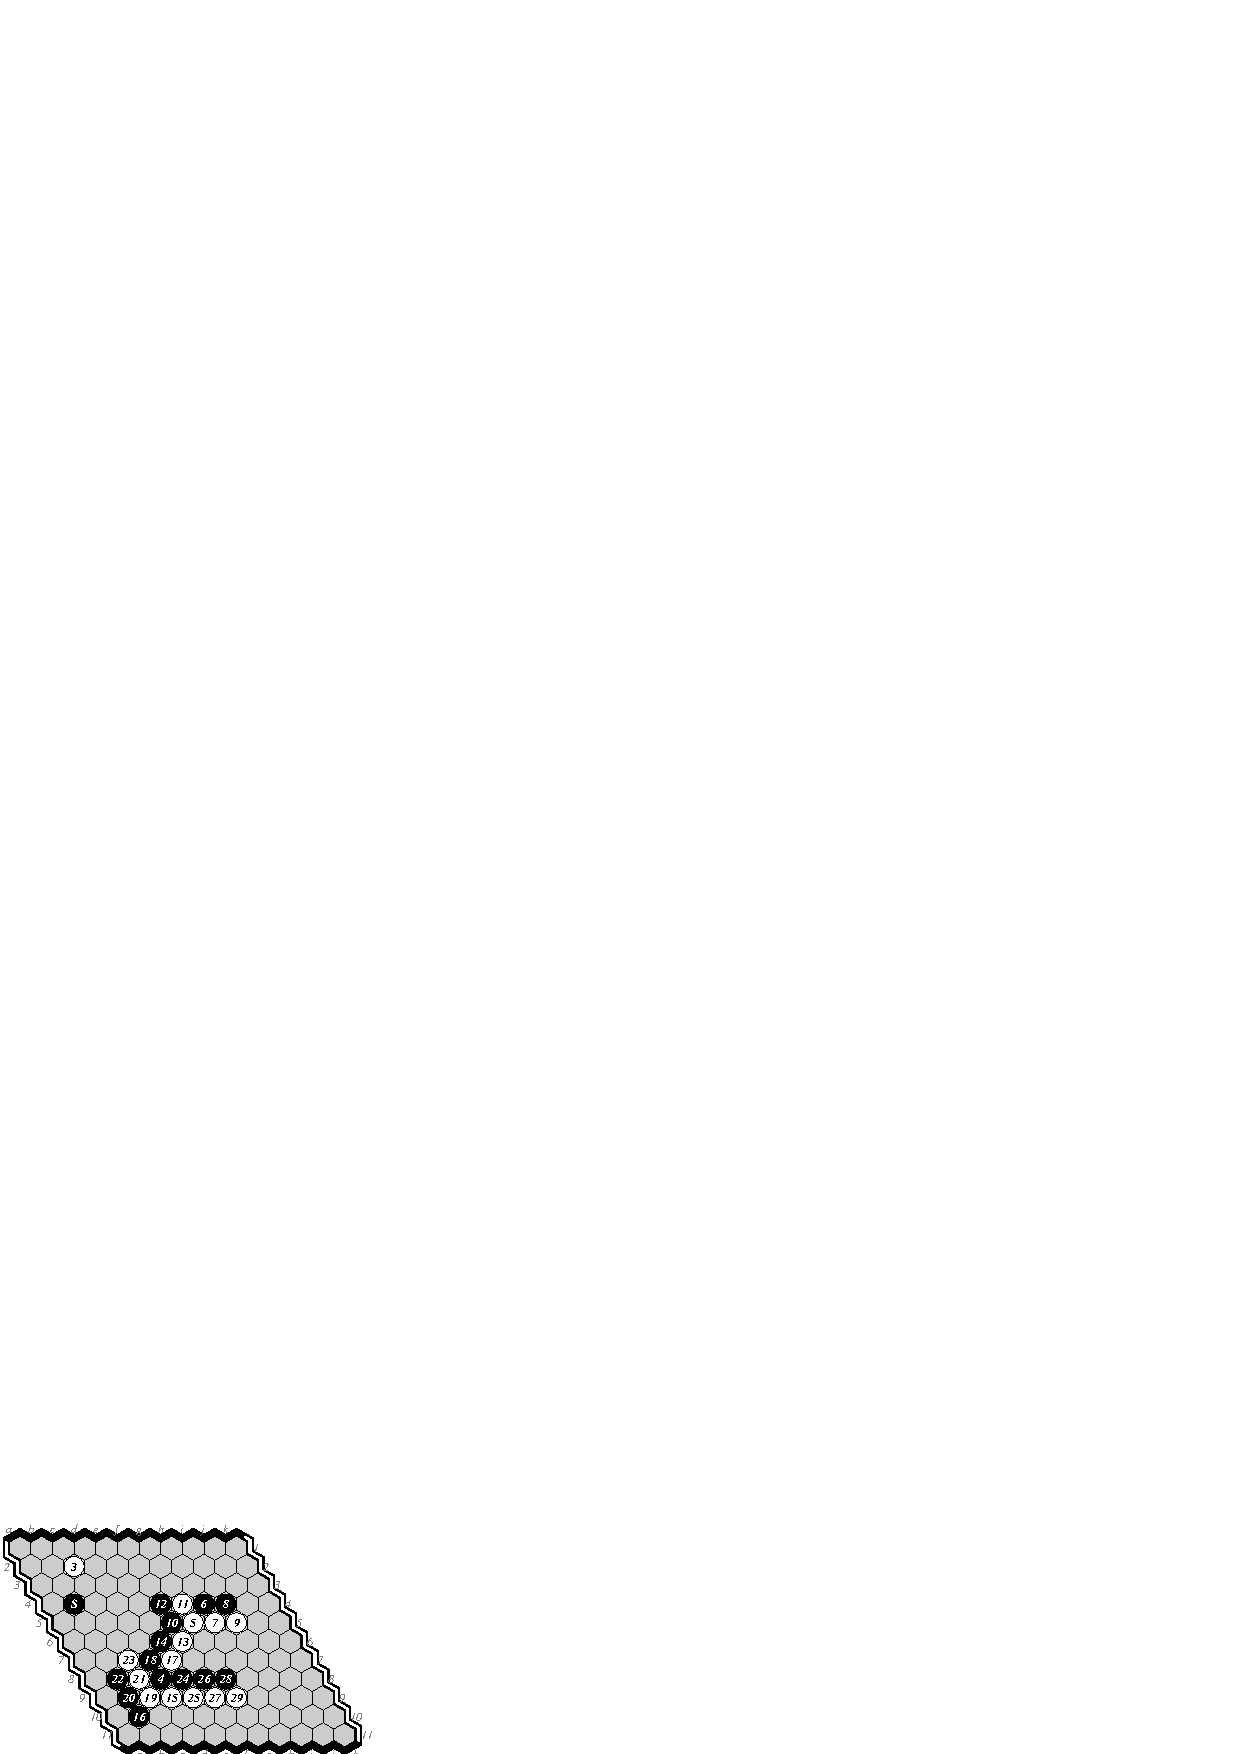
\includegraphics[width=.58\columnwidth]{pix/11-01-me}\hspace*{-.14\columnwidth}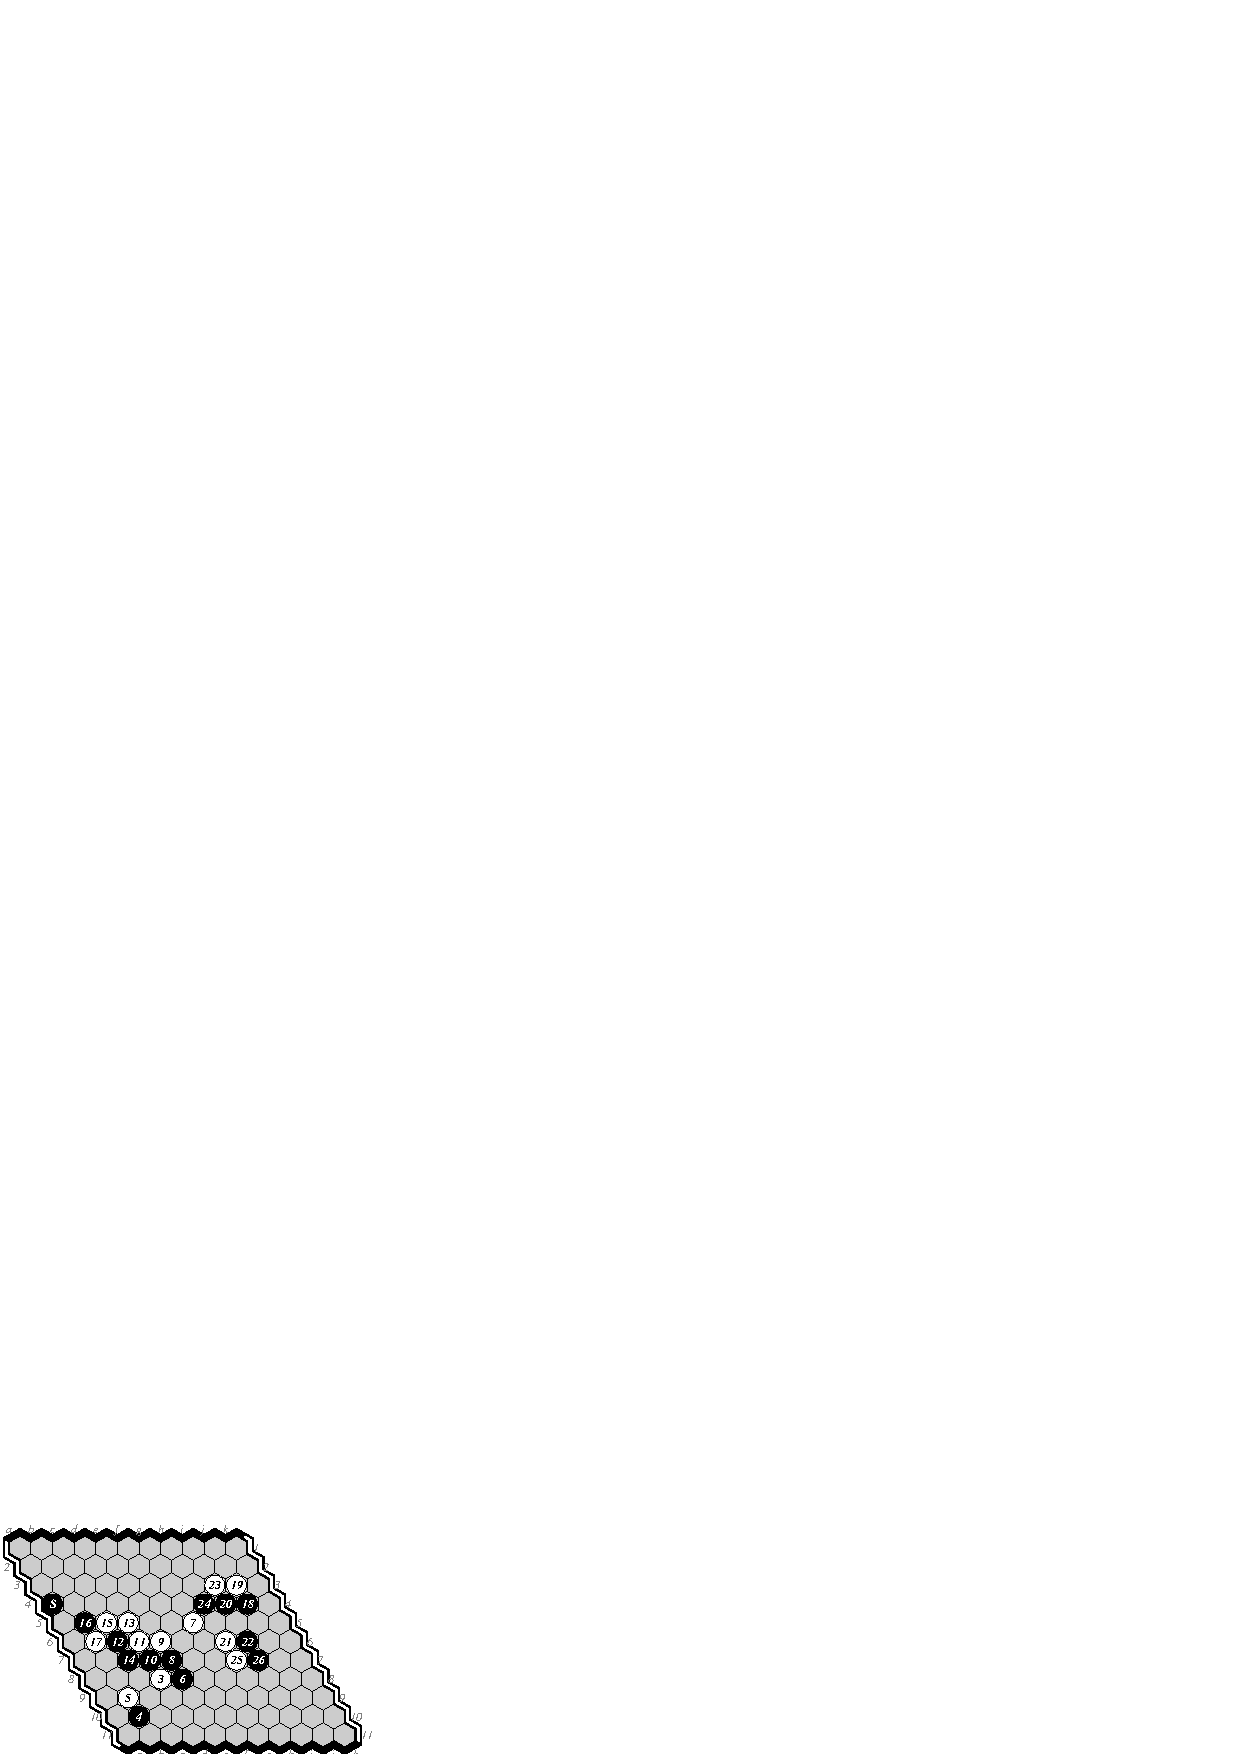
\includegraphics[width=.58\columnwidth]{pix/11-02-em}
\vspace*{.2cm}

\noindent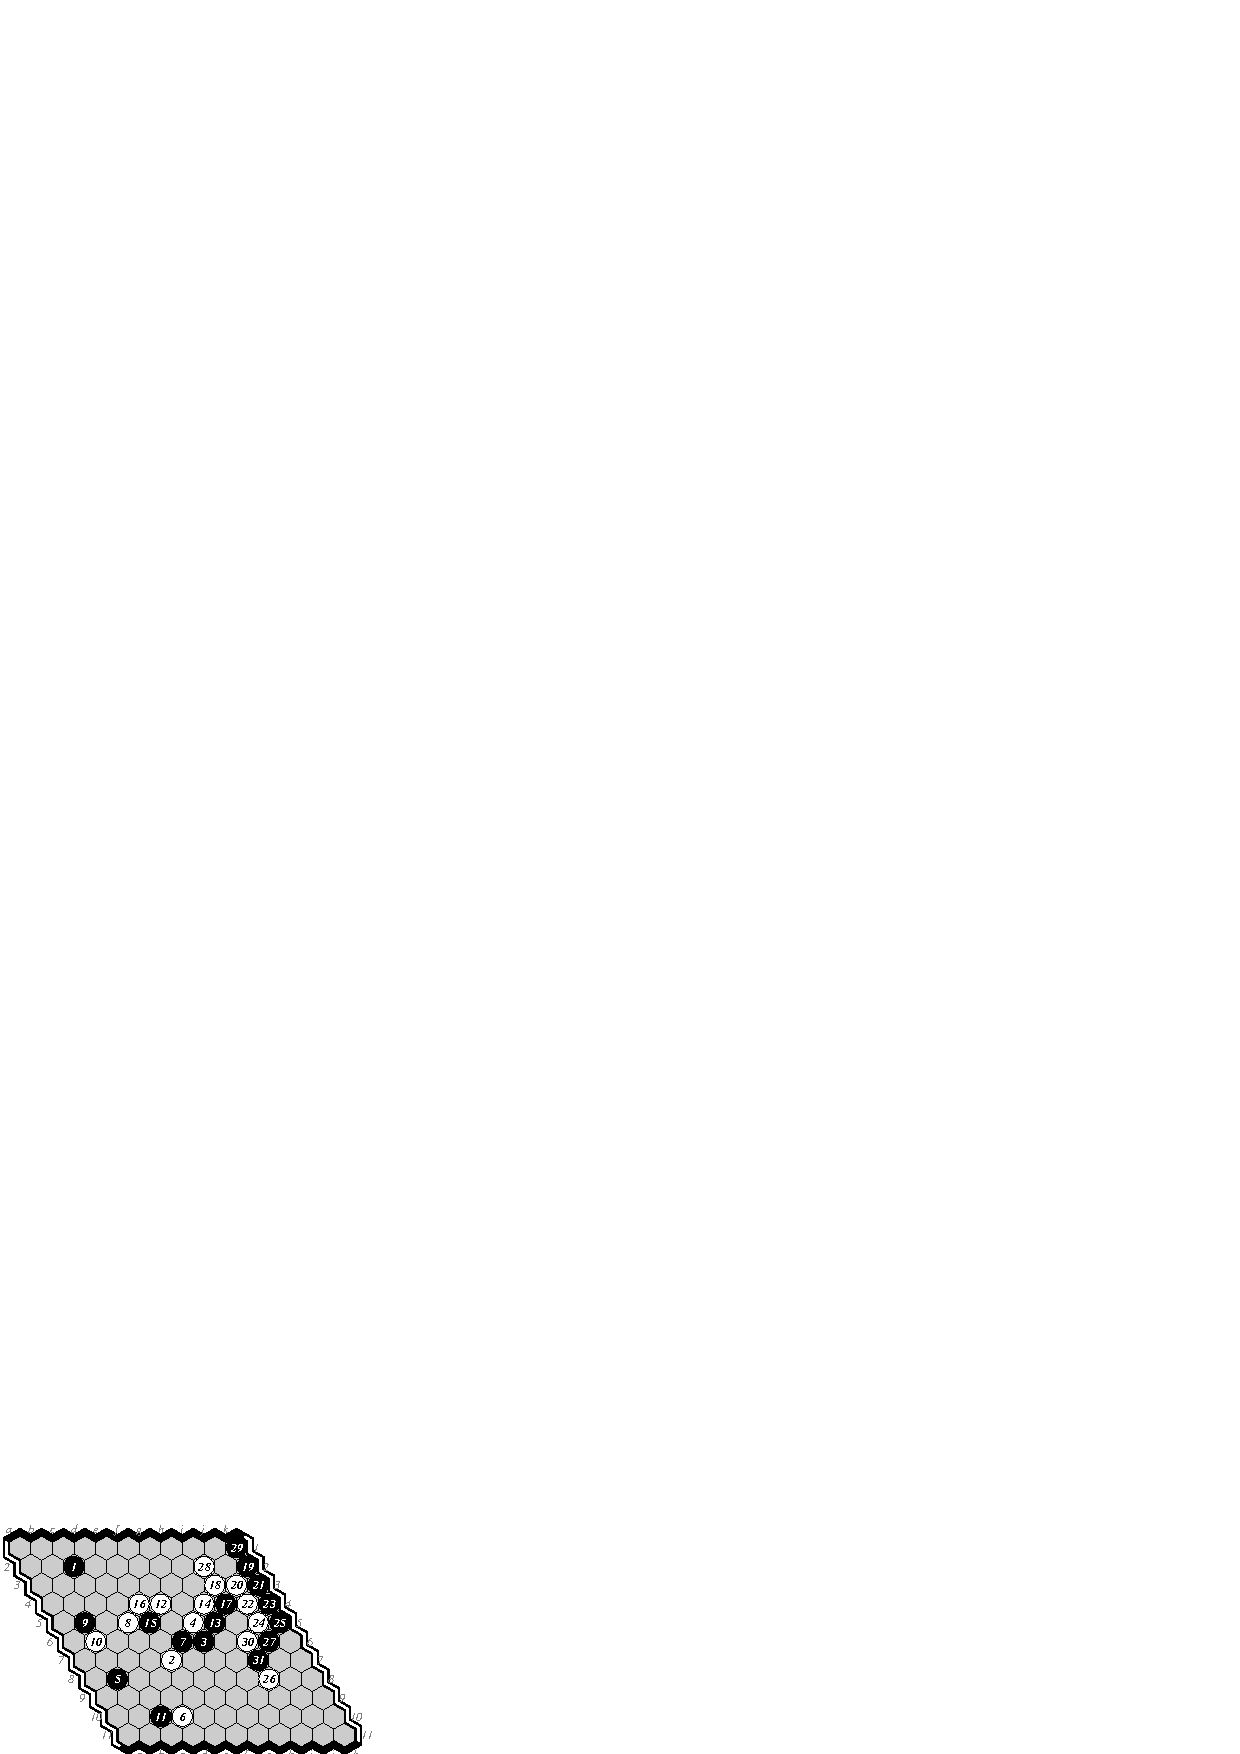
\includegraphics[width=.58\columnwidth]{pix/11-03-me}\hspace*{-.14\columnwidth}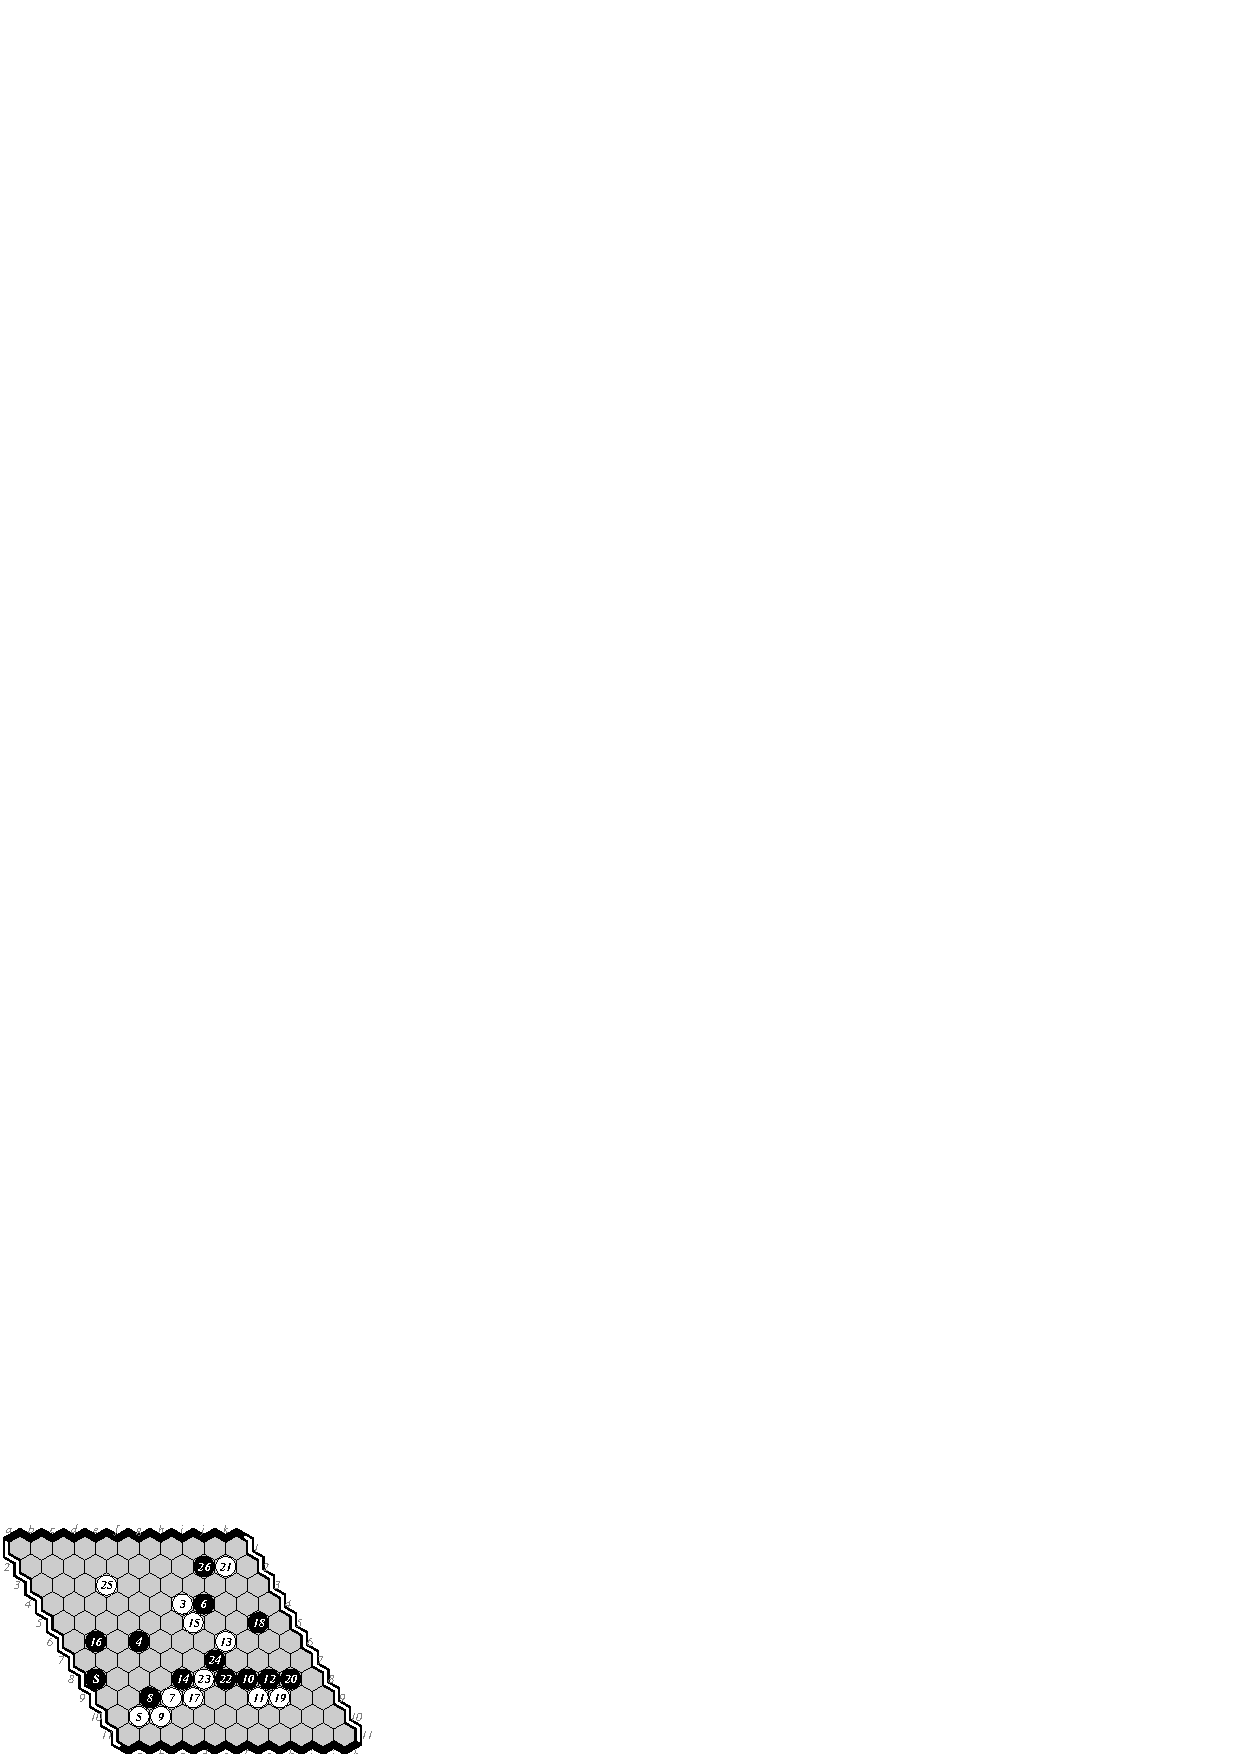
\includegraphics[width=.58\columnwidth]{pix/11-04-em}
\vspace*{.2cm}

\noindent\hfill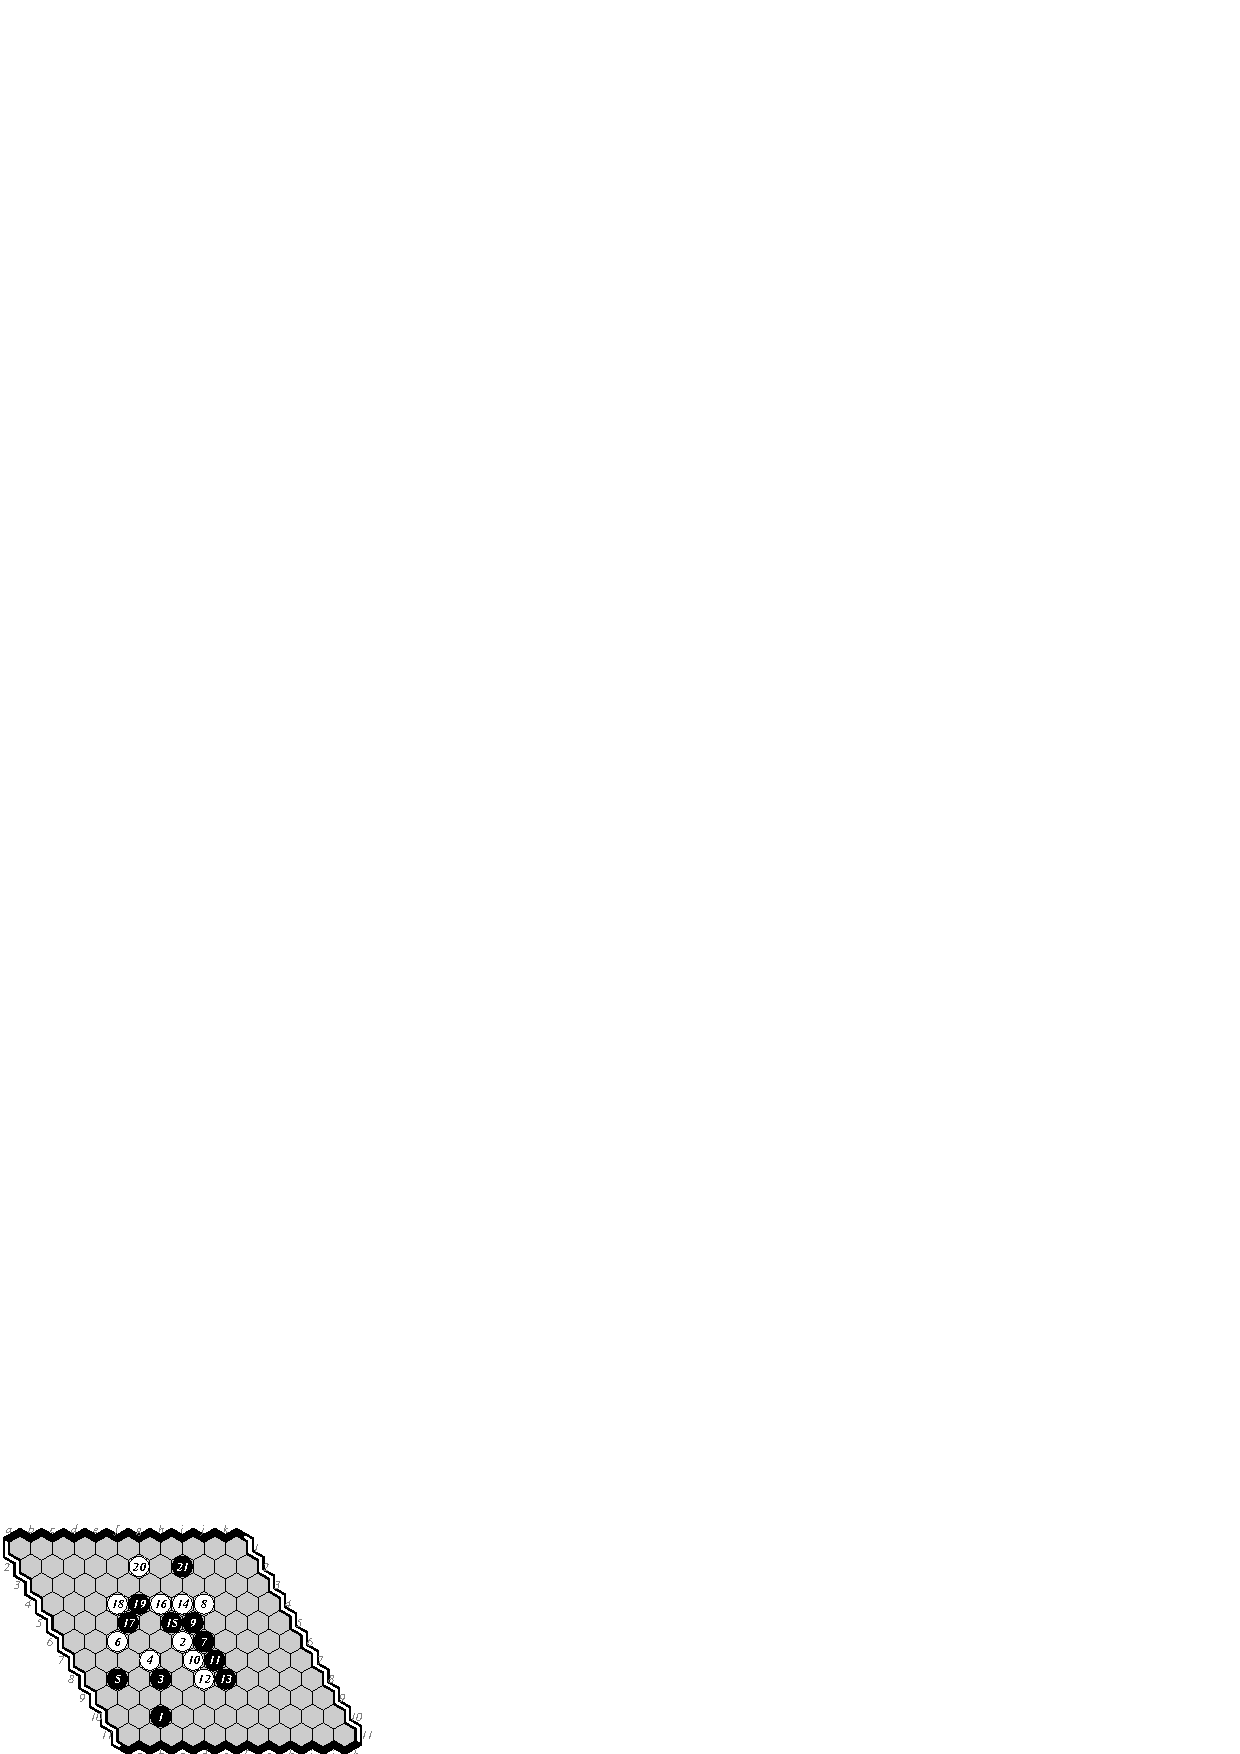
\includegraphics[width=.58\columnwidth]{pix/11-05-me}\hfill\ 
\caption{11$\times$11 Games 1-5. M-E 1-0, E-M 0-1, M-E 1-0, E-M 0-1, M-E 1-0.}
\end{figure}

\section{Conclusions}
here

\section*{Acknowledgements}
We thank the NSERC Discovery Grant Program for research funding.
\bibliographystyle{plain}
\bibliography{rpt}
\end{document}
